\documentclass[11pt]{article}
\usepackage[margin=1in]{geometry}
\usepackage{graphicx}
\usepackage{booktabs}
\usepackage{float}
\usepackage{amsmath}
\graphicspath{{figures/}}
\title{KernelAscent: RSI benchmark --- figure atlas}
\author{}
\date{\today}
\begin{document}
\maketitle
\noindent Auto-generated figure atlas (regenerate: \texttt{python3 scripts/make\_paper\_figures.py}). Pick the figures that matter; each has a \texttt{label} for cross-referencing.\par
\section{Leaderboards}
\begin{table}[H]\centering
\begin{tabular}{lrrr}
\toprule
Model & tier & rounds & $L-F$ \\
\midrule
starcoder2-15b & large & 6 & 0.232 \\
deepseek-coder-6.7b-base & mid & 3 & 0.154 \\
starcoder2-15b & large & 5 & 0.071 \\
deepseek-coder-1.3b-base & small & 12 & 0.039 \\
deepseek-coder-1.3b-base & small & 8 & 0.038 \\
Qwen2.5-Coder-1.5B & small & 2 & 0.038 \\
Qwen2.5-Coder-14B & large & 4 & -0.000 \\
Qwen2.5-Coder-1.5B & small & 2 & 0.000 \\
Qwen2.5-Coder-1.5B & small & 12 & 0.000 \\
Qwen2.5-Coder-7B & mid & 8 & 0.000 \\
Qwen2.5-Coder-7B & mid & 10 & 0.000 \\
deepseek-coder-1.3b-base & small & 3 & 0.000 \\
\bottomrule
\end{tabular}
\caption{Task 5 open self-play: author co-evolution $L-F$ leaderboard.}
\label{tab:t5}
\end{table}
\begin{table}[H]\centering
\begin{tabular}{lrrr}
\toprule
Model & $Q_0$ & $Q_g$ & $\Delta$ vs base \\
\midrule
us.openai.gpt-6-astra & 0.298 & 0.854 & 0.556 \\
us.anthropic.claude-sonnet-5 & 0.493 & 0.894 & 0.401 \\
mistral.mistral-large-3-675b & 0.359 & 0.669 & 0.310 \\
Nova-Pro & 0.401 & 0.490 & 0.089 \\
us.openai.gpt-5.6-sol & 0.813 & 0.889 & 0.075 \\
Kimi-K2.5 & 0.752 & 0.813 & 0.062 \\
Claude-Opus-5 & 0.878 & 0.910 & 0.032 \\
Fable-5.1 & 0.732 & 0.741 & 0.009 \\
us.openai.gpt-5.6-terra & 0.851 & 0.850 & -0.001 \\
Llama-3.3-70B & 0.458 & 0.455 & -0.004 \\
deepseek.v3.2 & 0.847 & 0.614 & -0.234 \\
\bottomrule
\end{tabular}
\caption{Task 3 procedure-RSI: held-out $Q$ gain vs.\ frozen procedure.}
\label{tab:t3}
\end{table}
\begin{table}[H]\centering
\begin{tabular}{lrrrr}
\toprule
Size band & $n$ & P(cross wall) & P(RSI) & mean drift \\
\midrule
<2B & 26 & 0.54 & 0.04 & 0.024 \\
2-8B & 17 & 0.94 & 0.41 & 0.299 \\
>=9B & 7 & 0.71 & 0.29 & 0.396 \\
\bottomrule
\end{tabular}
\caption{Scale $\to$ RSI gates: correctness-wall crossing and compounding by size band.}
\label{tab:gates}
\end{table}
\section{Mechanistic interpretability}
\begin{figure}[H]\centering
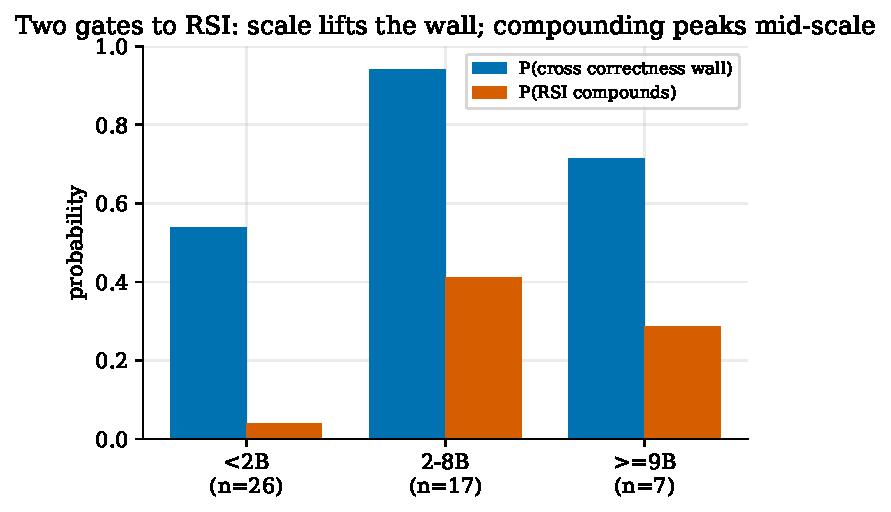
\includegraphics[width=0.86\linewidth]{mech_scale_gates.pdf}
\caption{Scale $\to$ RSI. Below $\sim$2B the correctness wall is rarely crossed, so weight-RSI is impossible; crossing rises sharply at 2B+, but compounding peaks at mid-scale (2--8B) and does not increase further $\geq$9B (headroom ceiling).}
\label{fig:mech_scale_gates}
\end{figure}
\begin{figure}[H]\centering
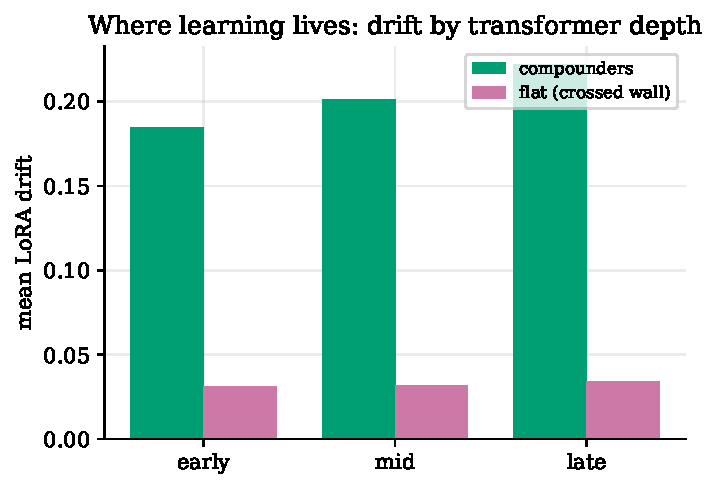
\includegraphics[width=0.86\linewidth]{mech_drift_by_depth.pdf}
\caption{LoRA weight drift by transformer depth for compounders vs.\ flat (wall-crossing) runs. Compounders sustain markedly larger drift across all depths; flat runs saturate early.}
\label{fig:mech_drift_by_depth}
\end{figure}
\begin{figure}[H]\centering
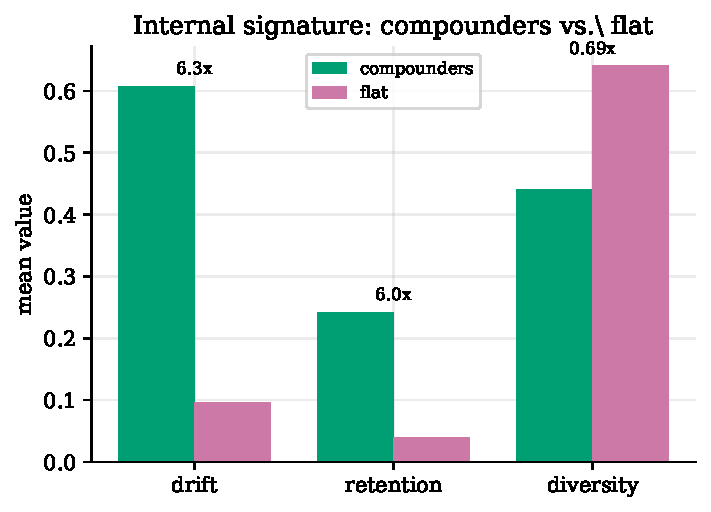
\includegraphics[width=0.86\linewidth]{mech_signature.pdf}
\caption{The internal signature that separates compounders from flat runs among wall-crossers: sustained drift and retention are $\sim$5--6$\times$ higher in compounders, while generation diversity is \emph{lower} (productive convergence, not diversity preservation).}
\label{fig:mech_signature}
\end{figure}
\begin{figure}[H]\centering
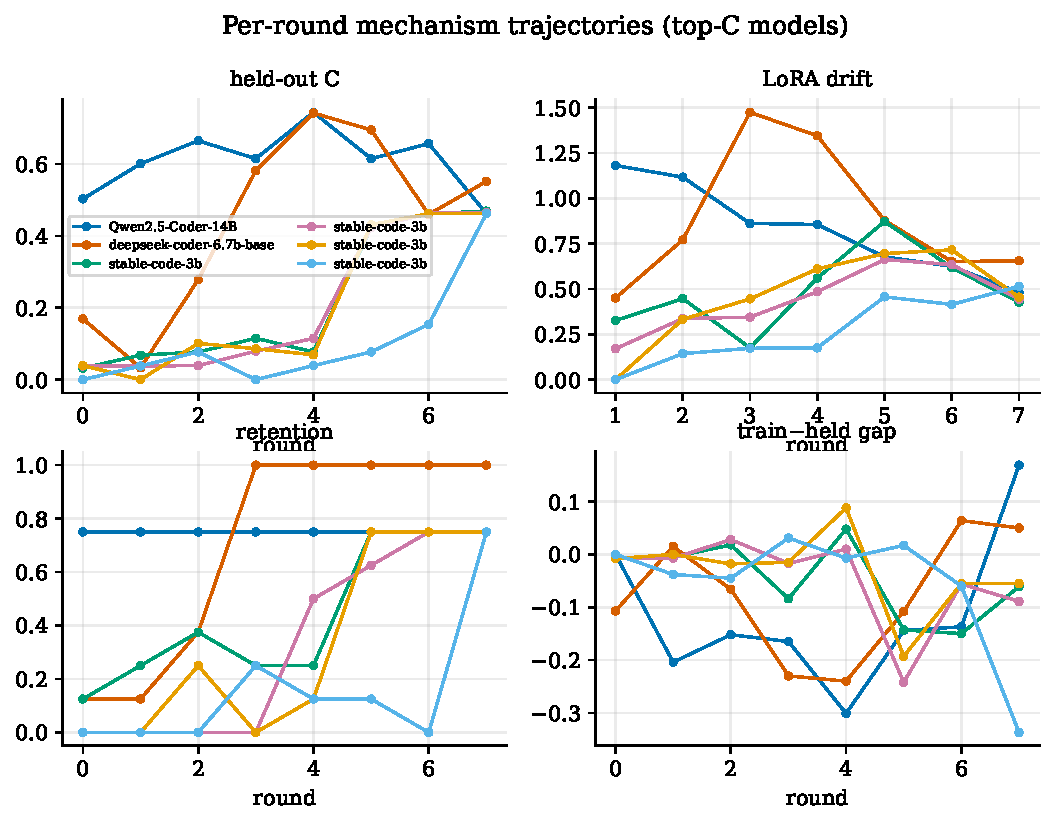
\includegraphics[width=0.86\linewidth]{mech_trajectories.pdf}
\caption{Per-round mechanism trajectories for the highest-capability probes: held-out C, total LoRA drift, retention, and the train$-$held transfer gap. Compounders show rising/held C with sustained drift and retention; flat runs plateau with drift saturation.}
\label{fig:mech_trajectories}
\end{figure}
\begin{figure}[H]\centering
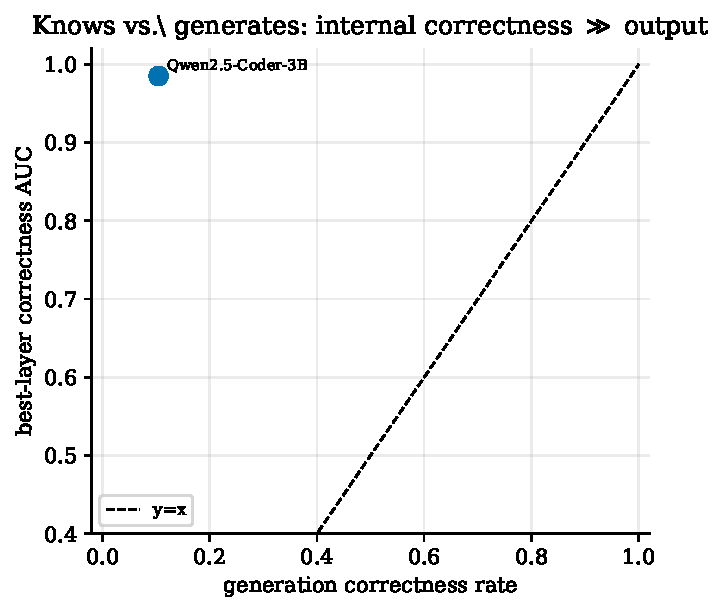
\includegraphics[width=0.86\linewidth]{interp_knows_vs_generates.pdf}
\caption{Internal correctness decodability (best-layer linear-probe AUC) vs.\ how often the model actually generates a correct kernel. Points far above $y=x$ mean the model \emph{represents} correctness internally far better than it can \emph{decode} it into a correct kernel: the RSI bottleneck is generation, not knowledge.}
\label{fig:interp_knows_vs_generates}
\end{figure}
\begin{figure}[H]\centering
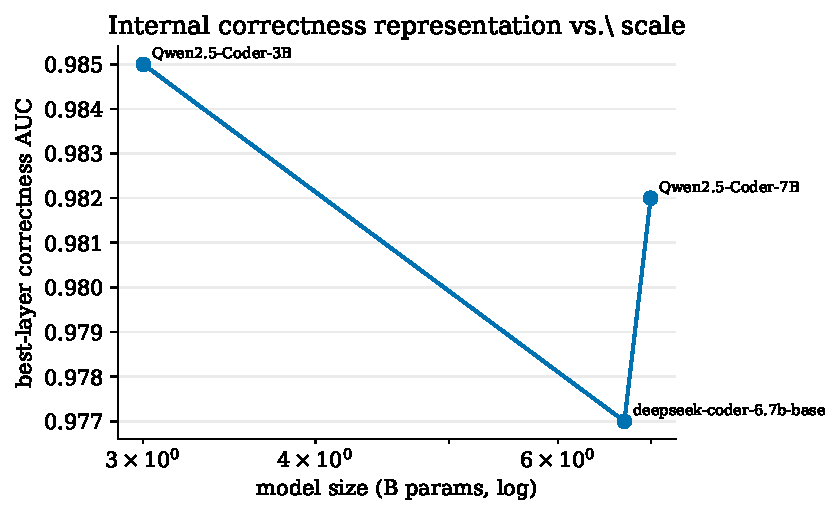
\includegraphics[width=0.86\linewidth]{interp_auc_vs_size.pdf}
\caption{Best-layer correctness-decodability AUC vs.\ model scale. (Populated as more interpretability probes land.)}
\label{fig:interp_auc_vs_size}
\end{figure}
\section{Task 5: self-play}
\begin{figure}[H]\centering
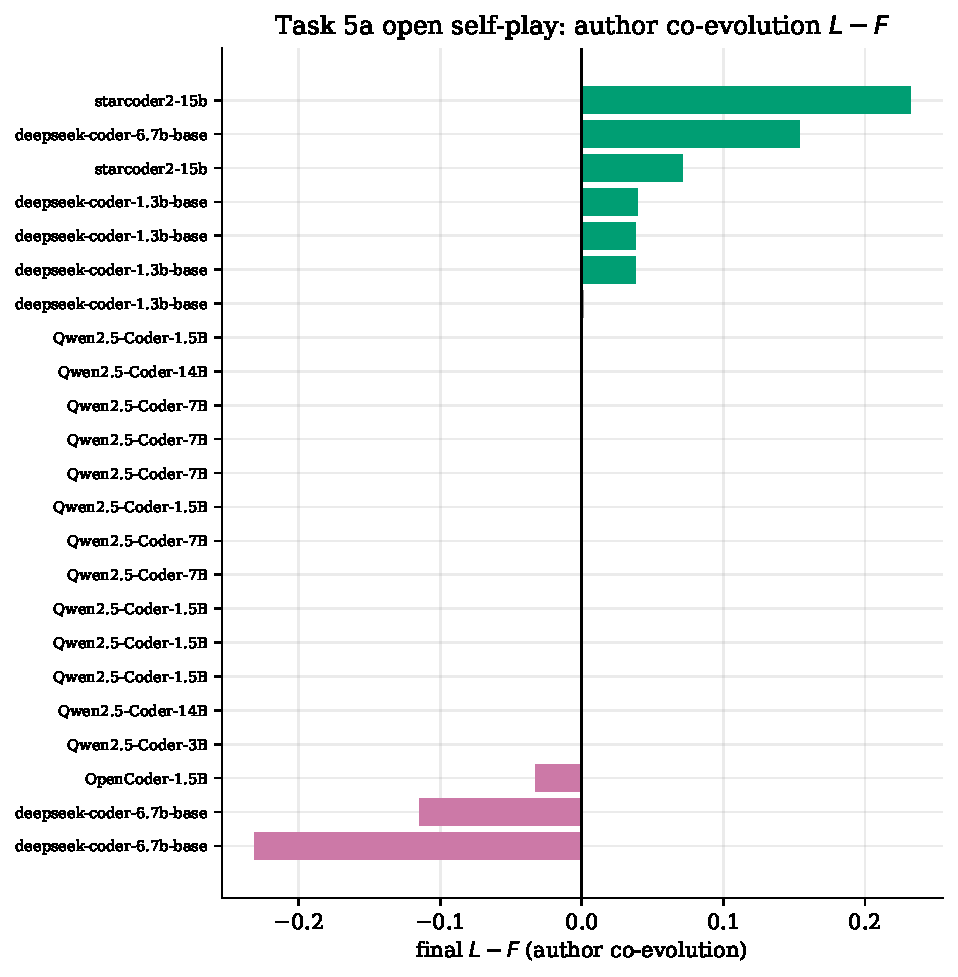
\includegraphics[width=0.86\linewidth]{t5_lf_open.pdf}
\caption{Final $L-F$ (live-author minus frozen-author, the self-referential signal) per open-weight model. $>0$ means updating the author beyond a frozen-author escalating curriculum genuinely helps.}
\label{fig:t5_lf_open}
\end{figure}
\begin{figure}[H]\centering
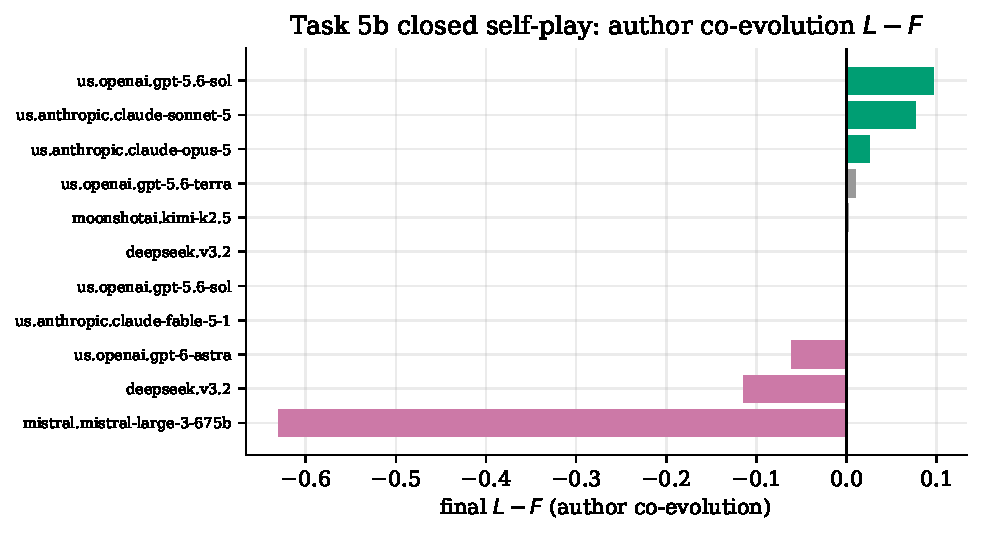
\includegraphics[width=0.86\linewidth]{t5_lf_closed.pdf}
\caption{Final $L-F$ per closed/API model (procedure co-evolution channel). Most cluster near zero; early large spikes did not survive longer horizons.}
\label{fig:t5_lf_closed}
\end{figure}
\begin{figure}[H]\centering
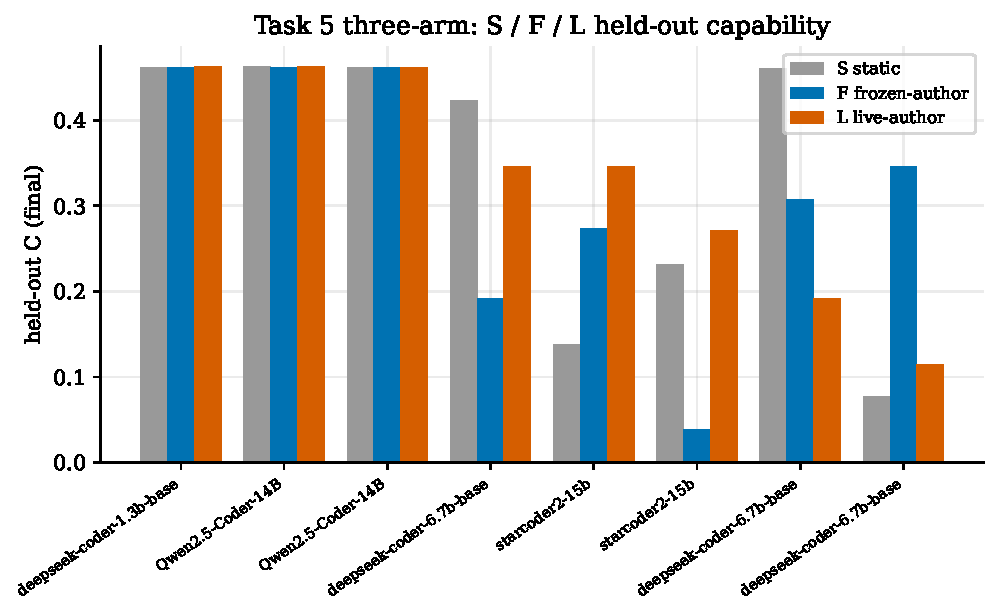
\includegraphics[width=0.86\linewidth]{t5_threearm.pdf}
\caption{Three-arm self-play at equal budget on a fixed held-out ladder: STATIC (fixed frontier), FROZEN-AUTHOR (escalating frontier, frozen base author), LIVE-AUTHOR (co-evolving author). $F-S$ isolates the adaptive-curriculum benefit; $L-F$ isolates author co-evolution.}
\label{fig:t5_threearm}
\end{figure}
\begin{figure}[H]\centering
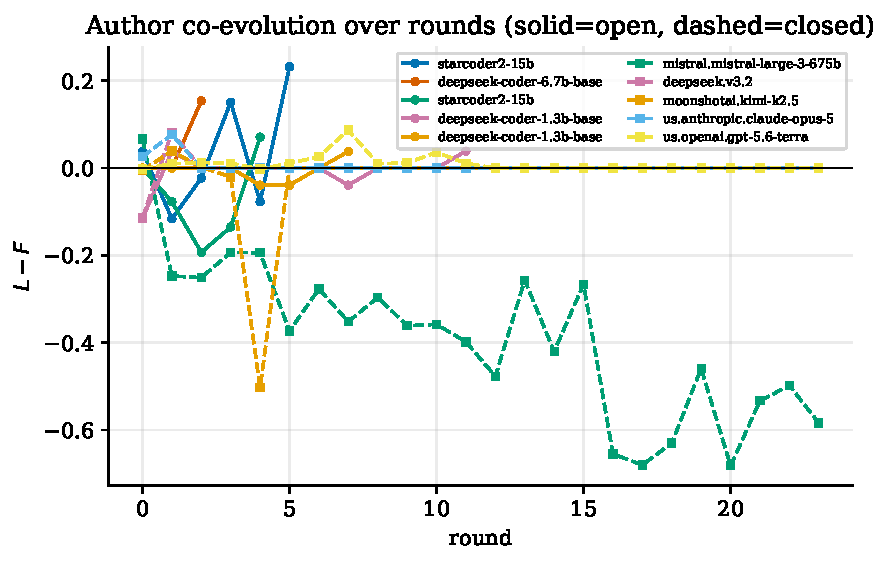
\includegraphics[width=0.86\linewidth]{t5_lf_trajectory.pdf}
\caption{Per-round $L-F$ trajectories (solid = open-weight, dashed = closed/API). Long horizons reveal whether early positive spikes compound or regress to zero.}
\label{fig:t5_lf_trajectory}
\end{figure}
\begin{figure}[H]\centering
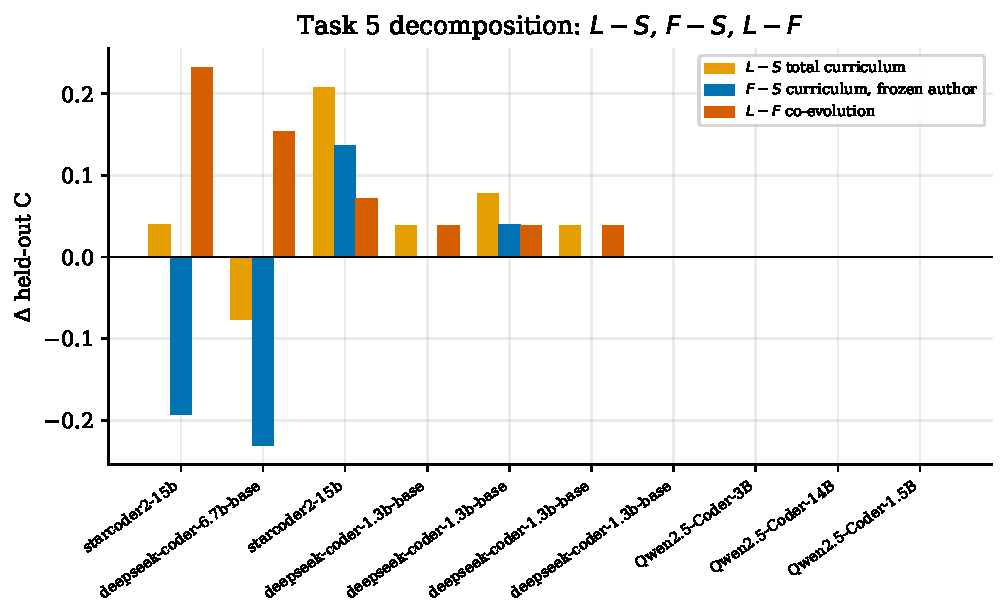
\includegraphics[width=0.86\linewidth]{t5_decomposition.pdf}
\caption{Decomposing the self-play benefit: $L-S$ (total adaptive-curriculum gain) $=$ $(F-S)$ (curriculum with a frozen author) $+$ $(L-F)$ (extra gain from co-evolving the author). Most models get their gain from $F-S$, not $L-F$.}
\label{fig:t5_decomposition}
\end{figure}
\begin{figure}[H]\centering
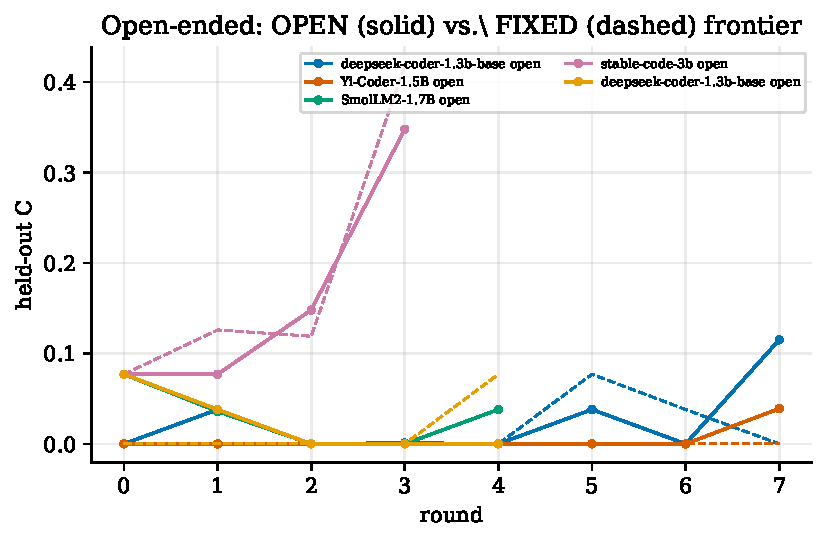
\includegraphics[width=0.86\linewidth]{t5_openended.pdf}
\caption{Open-ended RSI: a learner facing an OPEN escalating self-authored frontier (solid) vs.\ a FIXED static frontier (dashed) at equal budget. Overlap means open-endedness is a one-time upgrade, not compounding.}
\label{fig:t5_openended}
\end{figure}
\section{Task 4: closed$\to$open}
\begin{figure}[H]\centering
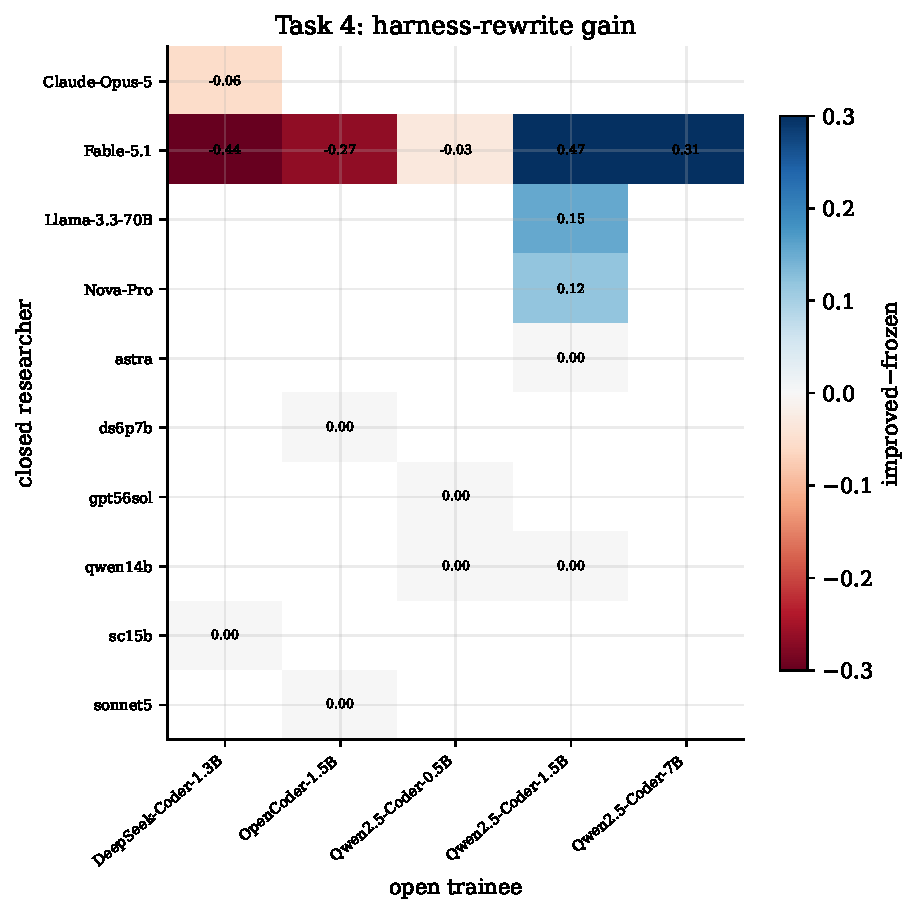
\includegraphics[width=0.86\linewidth]{t4_heatmap.pdf}
\caption{Task 4 (closed$\to$open): a closed frontier researcher rewrites an open trainee's training harness. Cell = improved$-$frozen held-out C on the trainee (positive = the rewritten harness helps).}
\label{fig:t4_heatmap}
\end{figure}
\begin{figure}[H]\centering
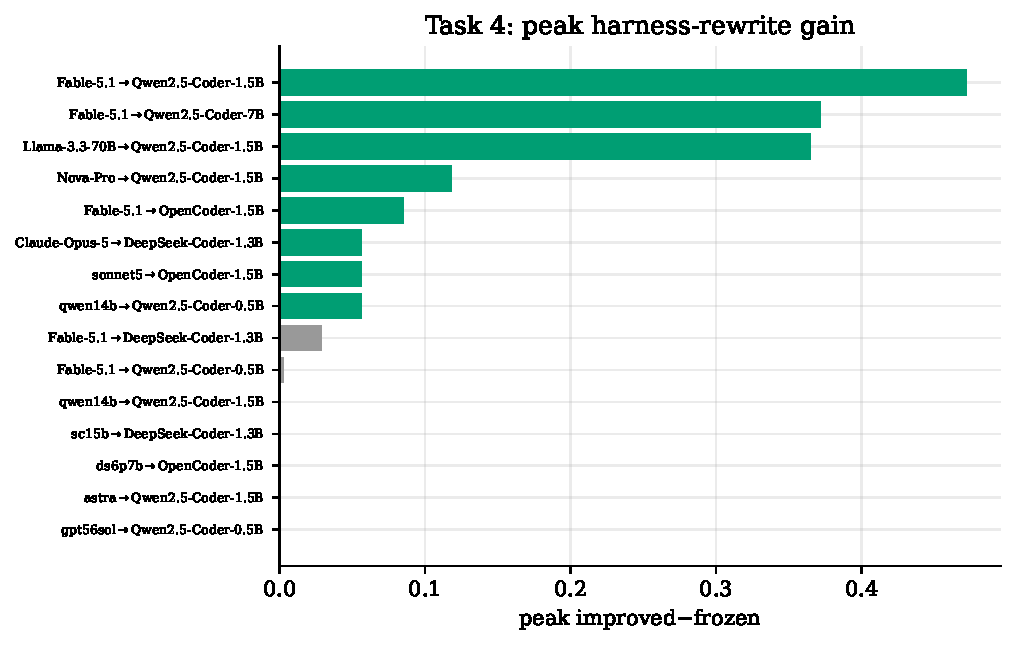
\includegraphics[width=0.86\linewidth]{t4_peak.pdf}
\caption{Peak improved$-$frozen over rounds for each researcher$\to$trainee pair.}
\label{fig:t4_peak}
\end{figure}
\section{Task 3: procedure-RSI}
\begin{figure}[H]\centering
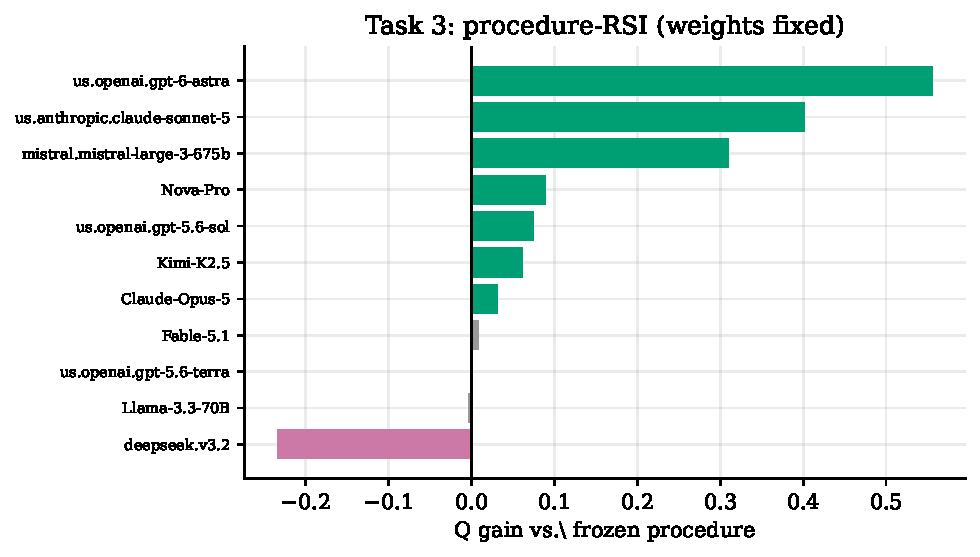
\includegraphics[width=0.86\linewidth]{t3_procedure_rsi.pdf}
\caption{Task 3: a frozen-weight model rewrites its own strategy library + verified archive. Held-out Q gain vs.\ the frozen procedure; frontier models improve their own procedure substantially.}
\label{fig:t3_procedure_rsi}
\end{figure}
\section{Comparators \& weight-RSI}
\begin{figure}[H]\centering
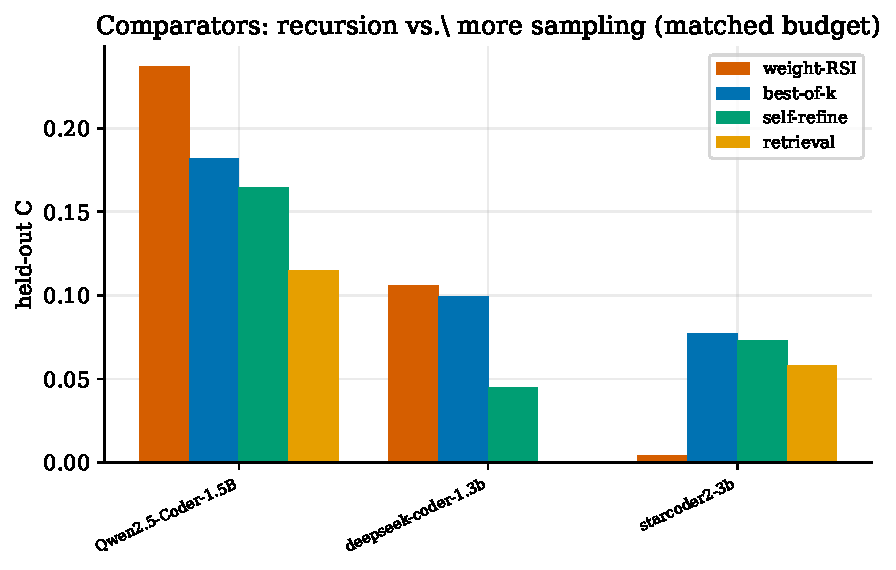
\includegraphics[width=0.86\linewidth]{cmp_recursion_gain.pdf}
\caption{Is it really recursion? Weight-RSI vs.\ non-recursive controls (best-of-k, self-refine, retrieval) at matched generation budget. recursion\_gain $=$ weight-RSI $-$ best comparator.}
\label{fig:cmp_recursion_gain}
\end{figure}
\begin{figure}[H]\centering
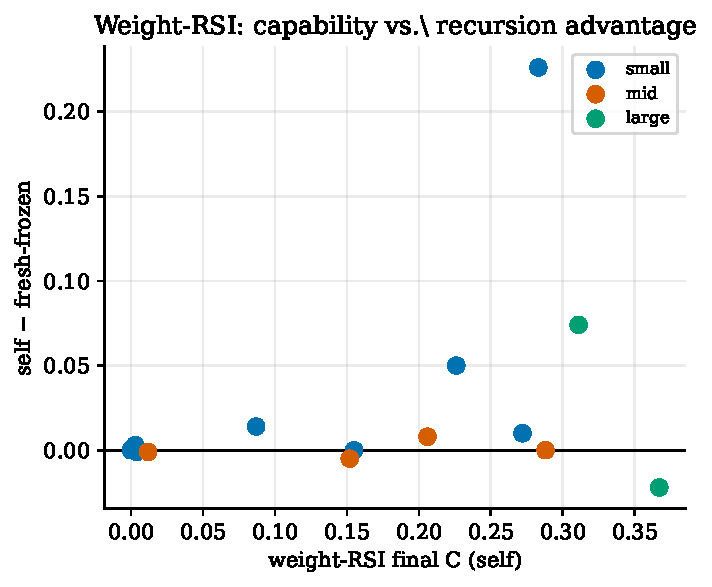
\includegraphics[width=0.86\linewidth]{t2_selfvsfresh.pdf}
\caption{Weight-RSI: final self-trained held-out C vs.\ the self-minus-fresh-frozen advantage (positive = training on own kernels beats an equal-budget fresh baseline).}
\label{fig:t2_selfvsfresh}
\end{figure}
\begin{figure}[H]\centering
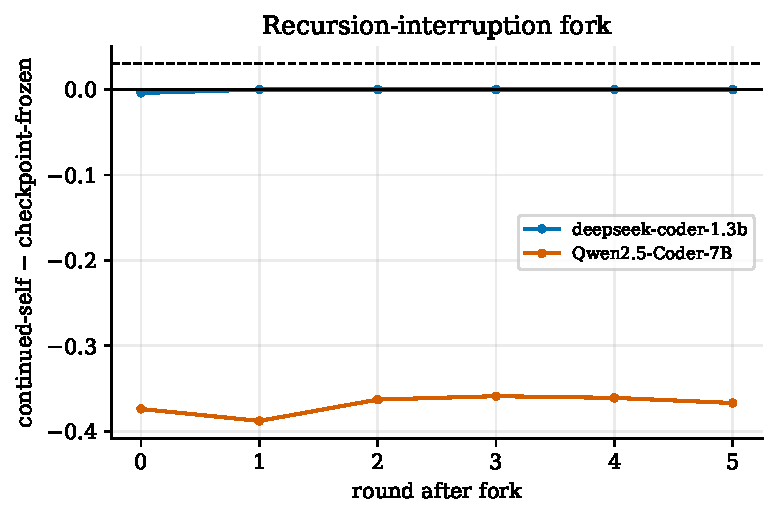
\includegraphics[width=0.86\linewidth]{fork_recursion.pdf}
\caption{Recursion-interruption control: continued self-training vs.\ a checkpoint-frozen producer at equal budget. Sustained $>0$ = genuine compounding rather than a one-time producer upgrade.}
\label{fig:fork_recursion}
\end{figure}
\section{Flows \& causality}
\begin{figure}[H]\centering
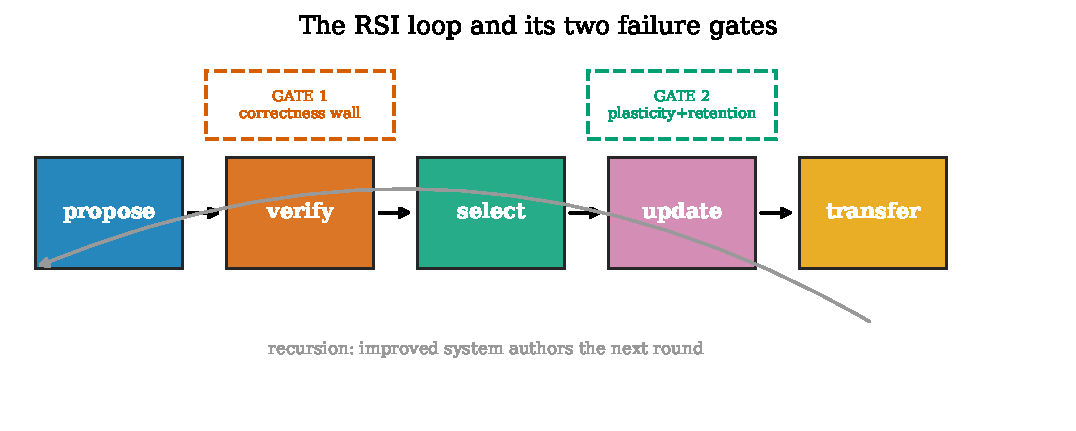
\includegraphics[width=0.86\linewidth]{flow_rsi_loop.pdf}
\caption{The recursive self-improvement loop (propose$\to$verify$\to$select$\to$update$\to$transfer) and the two gates our data identifies: Gate 1, the correctness wall (no verified kernel $\Rightarrow$ no gradient), and Gate 2, plasticity+retention (drift saturation / forgetting collapses compounding).}
\label{fig:flow_rsi_loop}
\end{figure}
\begin{figure}[H]\centering
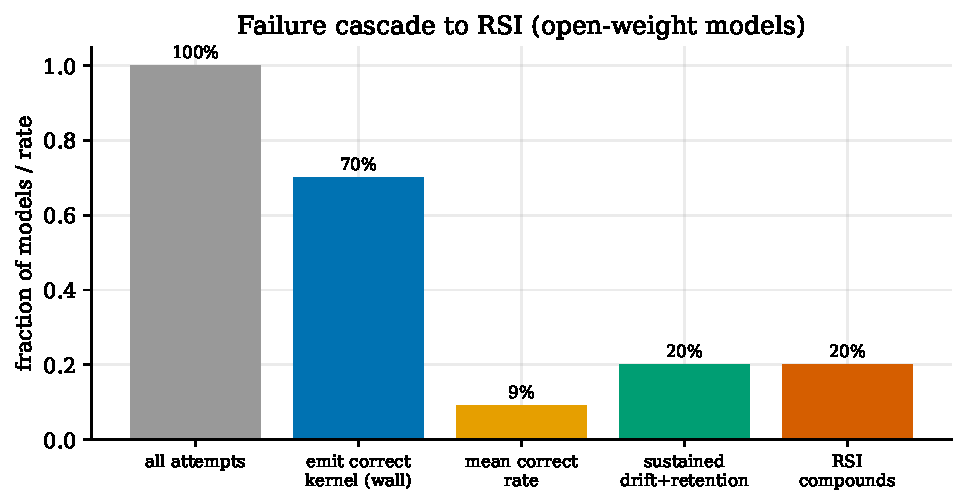
\includegraphics[width=0.86\linewidth]{flow_failure_cascade.pdf}
\caption{Attrition from attempt to compounding RSI across open-weight models: most attrition happens at the correctness wall (emitting any correct kernel) and again at sustained plasticity+retention.}
\label{fig:flow_failure_cascade}
\end{figure}
\begin{figure}[H]\centering
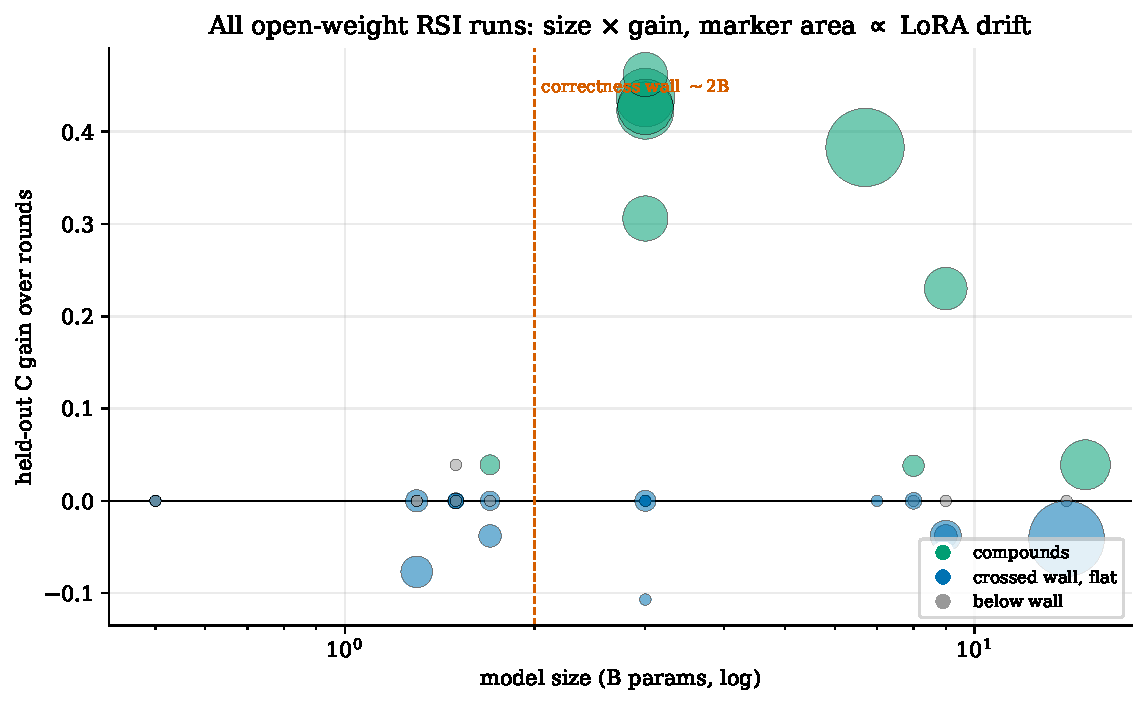
\includegraphics[width=0.86\linewidth]{flow_all_runs.pdf}
\caption{Every open-weight weight-RSI run positioned by model size ($x$) and held-out C gain ($y$); marker area $\propto$ sustained LoRA drift; color = outcome. The 2B correctness wall and the mid-scale compounding band are visible at a glance.}
\label{fig:flow_all_runs}
\end{figure}
\end{document}